As described in Section~\ref{sec:physics-lbnosc-senscalc}, the effect of systematic uncertainty on
experimental sensitivity is approximated by allowing the neutrino oscillation
parameters to vary within the uncertainty in the global fit to neutrino data
\cite{Gonzalez-Garcia:2014bfa} and by allowing the  signal and background rates
to vary based on normalization uncertainties. In the sensitivities presented there,
the \nue and \anue signal normalization uncertainties are $5\% \oplus 2\%$, implemented as
5\% signal normalization uncertainties on the \numu and \anumu samples and
2\% on the \nue and \anue samples. These four signal normalization uncertainties
are treated as 100\% uncorrelated so that the 2\% normalization uncertainty on the
\nue sample represents a residual normalization uncertainty after constraints
from the near detector, the \numu disappearance samples, and the \anue sample have been applied.
The normalization uncertainties on background to these samples and the correlation among those
uncertainties are presented in Table~\ref{tab:bgnormsys}. The result of the correlations
presented in Table~\ref{tab:bgnormsys} is that there are five independent background
normalization uncertainties: beam \nue, beam \anue, \numu/NC background to appearance mode,
NC background to disappearance mode, and $\nu_\tau$.

\begin{table}[!tb]
  \begin{center}
    \caption{Normalization uncertainties and correlations for background to the \nue, \anue, \numu, and \anumu data samples.}
    \label{tab:bgnormsys}
    \begin{tabular}{l|c|l} \hline\hline
      Background & Normalization Uncertainty & Correlations \\ \hline
      \multicolumn{3}{l}{For \nue/\anue appearance:} \\ 
      Beam \nue & 5\% & Uncorrelated in \nue and \anue samples \\
      NC      & 5\%  & Correlated in \nue and \anue samples \\
      \numu CC & 5\% & Correlated to NC \\
      $\nu_\tau$ CC & 20\% & Correlated in \nue and \anue samples \\ \hline
      \multicolumn{3}{l}{For \numu/\anumu disappearance:} \\ 
      NC & 5\% & Uncorrelated to \nue/\anue NC background \\
      $\nu_\tau$ & 20\% & Correlated to \nue/\anue $\nu_\tau$ background \\
    \end{tabular}
  \end{center}
  \end{table}

In this section, we present a justification for the chosen values of the signal and background
normalization uncertainties and we consider the effect of varying the size of the residual normalization
uncertainties on the \nue and \anue samples.We also describe the ongoing effort to characterize and evaluate the effect of individual sources
of uncertainty in the DUNE experiment.

\subsection{Effect of Normalization Uncertainties}
Figure \ref{fig:exp_systs} shows the
change in DUNE sensitivity to neutrino mass hierarchy and discovery of CP violation
as a function of exposure for several levels of this uncertainty.
As seen in Fig.~\ref{fig:exp_systs}, for early phases of DUNE
with exposures less than 100 kt-MW-years, the experiment
will be statistically limited. In the full experiment, signal and
background normalization uncertainties remain
relatively unimportant for the mass hierarchy measurement, when considering
minimum sensitivity for 100\% of \deltacp values, because the minimum sensitivity 
occurs in the near-degenerate region where \deltacp is near $\pi/2$. In this
region, much of the sensitivity to mass hierarchy comes from spectral analysis of
the oscillations and is therefore less sensitive to normalization uncertainty.
It is important to note that the sensitivity calculations presented here do not
consider the effect of energy scale uncertainty, which may have a more significant
impact on mass hierarchy sensitivity. Studies of the impact of energy scale 
uncertainty are in progress and will be included in future analyses of experimental
sensitivity. The impact of systematic uncertainty on the CP violation sensitivity
is obvious in Fig.~\ref{fig:exp_systs}; the \nue signal normalization uncertainty must
be understood at the level of $5\% \oplus 2\%$ in order to reach 5$\sigma$ sensitivity for exposures less 
than xxx kt-MW-years. Specifically,
the absolute normalization of the \numu sample must be known to $\sim$5\% and
the normalization of the \nue sample,
relative to the \anue, \numu, and \anumu samples after all constraints from
external, near detector, and far detector data have been applied, must be determined 
at the few percent level.
% \begin{figure}[!htbp]
% \centering
% \includegraphics[width=0.45\linewidth]{figs/MHSigFrac_lbne_SBGErrs.pdf}
% \includegraphics[width=0.45\linewidth]{figs/CPVSigFrac_lbne_SBGErrs.pdf}
% \caption{Expected sensitivity of DUNE to determination of the neutrino mass
%   hierarchy (left) and discovery of CP violation, i.e. $\dcp \ne$ 0 or $\pi$,
%   (right) as a function of exposure in kt-MW-years, assuming 
%   equal running in neutrino and antineutrino mode, for a range of values for
%   the residual \nue and \anue signal and
%   background normalization uncertainties. The sensitivities quoted
%   are the minimum sensitivity for 100\% of \deltacp values in the case of 
%   mass hierarchy and 50\% of \deltacp values in the case of CP violation.
%   Sensitivities are for true normal hierarchy; neutrino mass hierarchy is assumed to
%   be unknown in the CPV fits.}
% \label{fig:exp_systs}
% \end{figure}

\subsection{Justification of Normalization Uncertainties}
\label{sec:syst_just}
Uncertainties in DUNE
will be constrained by external data, near detector data, and the combined
fit to the four (\nue, \anue, \numu, \anumu) far detector samples.  
Experience from previous and currently-running neutrino oscillation 
experiments suggests that $5\% \oplus 2\%$
signal normalization (where 5\% is the normalization uncertainty on the
FD \numu sample and 2\% is the residual uncorrelated uncertainty on the
FD \nue sample after all constraints) and normalization uncertainties on
background as given in Table \ref{bgnormsys}
are reasonably achievable in DUNE given a capable near detector with argon targets.
Table~\ref{tab:nuesysts} shows the uncertainties in a \nue appearance
analysis achieved by MINOS~\cite{Adamson:2013ue} 
and T2K~\cite{Abe:2015awa} and compares the 
expected uncertainty in
DUNE. The goal uncertainties in DUNE are chosen by determining which
of the existing experiments is more representative of DUNE for each source
of systematic uncertainty and then setting the reasonable goal that a next
generation experiment, with the high resolution of a LAr TPC and precise measurements
from a highly capable near detector, should be able to improve on a similar earlier experiment.
A brief explanation of each choice in Table~\ref{tab:nuesysts} follows.
\subsubsection{Flux Uncertainties}
\label{sec:syst_just_flux}
DUNE plans to take advantage of spectral analysis,
meaning that absolute and relative flux normalization is required. Since the MINOS \nue appearance analysis
is based on normalization only, in terms of the \nue appearance analysis, DUNE will be more like T2K,
which has achieved 3.2\% normalization uncertainty on their \nue sample due to flux. Additionally, for a more apt
comparison to MINOS performance, the inclusive neutrino charged current cross-section measurement from the MINOS
near detector reported in \cite{xxx} has acheived a normalization uncertainty of $\sim$2\% in the
range $3 < E_\nu < 9$ GeV and the near-to-far \numu unoscillated-spectrum extraplolation errors in MINOS
are $<$3\% without any independent constraints on hadron production or muon flux measurements at the near
site. Therefore, as DUNE is planned to have a highly capable near detector, beam line
muon detectors, dedicated hadronization measurements, and improved simulation of beam flux based on MINERvA
measurements in the NuMI beam, we set a goal uncertainty on \nue signal
normalization from uncertainties in the flux determination of 2\%.
As described in Section \ref{sec:syst_studies_ind}, preliminary
studies of the FGT ND support this estimate, predicting 2\% uncertainty on the absolute flux and 1-2\%
uncertainty on the flux shape.
\subsubsection{Simulation Uncertainties}
\label{sec:syst_just_sim}
This category of uncertainties arise primarily from uncertainties in modeling neutrino interactions with the target
nuclei in the near and far detectors. These uncertainties include \nue and \numu cross-section uncertainties,
uncertainties from modeling the structure of the target nucleus, and the impact of
hadronization model uncertainties in simulating the break up of the target nucleus in higher-energy inelastic
interactions. DUNE will employ argon nuclear targets in both the near and far detectors, allowing for a larger
cancellation of simulation uncertainties than in T2K, in which the target nuclei in the near detector are
carbon while those in the far detector are oxygen, and making comparison to MINOS, which also employed identical
nuclei (iron) in the near and far detectors, most appropriate. MINOS achieved a 2.7\% residual uncertainty on
the \nue signal after constraints from the near detector were applied. DUNE's high-resolution near
detector is expected to enable further constraints on hadronization uncertainties, relative to MINOS, by
resolving many of the individual particles produced in the resonance and deep-inelastic scattering interactions
which represent the majority of the DUNE data sample. Therefore, we take 2\% as a goal for the effect of
simulation uncertainties on DUNE \nue signal normalization. It is important to note that this level of
uncertainty depends upon the ability to isolate neutrino-argon interactions in the near detector to facilitate
cancellation of near-far uncertainties; this is a requirement of the ND design.

Additionally, in considering the effect of the three-flavor analysis on the final uncertainty,
the neutrino beams in DUNE and MINOS have energy
spectra that peak around 2.5-3.0~GeV, compared to 600~MeV in T2K. The relatively large uncertainty
in the ratio of \nue/\numu cross-sections in T2K will be significantly lower at DUNE energies,
increasing the level of cancellation that can be expected in the three-flavor analysis. As
described in Section~\ref{sec:syst_studies_ind}, preliminary studies with a Fast MC demonstrate the
expected cancellation of cross-section uncertainties in the DUNE three-flavor analysis.

\subsubsection{\nue Energy Scale Uncertainties}
\label{sec:syst_just_fd}
MINOS and T2K have acheived uncertainty in the \nue signal normalization from \nue energy scale
of 2.7\% and 2.5\% respectively,
where the 2.5\% from T2K actually includes most far detector effects. DUNE's LAr TPC far detector
is expected to outperform both the MINOS sampling calorimeter and the T2K water Cerenkov detector
in reconstruction of \nue interactions. Significant experience with simulation, reconstruction, and calibration
of neutrino interactions in LAr TPCs is expected from the Intermediate Neutrino Program, particularly
Fermilab's SBN program which will include three LAr TPCs: SBND, $\mu$BooNE, and ICARUS. An active program of
prototypes and test beam measurements is planned to study the reconstruction of charged and neutral particles
in LAr TPCs; this suite of experiments includes the DUNE 35-ton prototype, LArIAT, CAPTAIN, and
the CERN neutrino platform single and dual phase prototypes.
Therefore, we set a goal of using the superior detector performance and the improvments
in understanding of LAr TPC energy response expected in the next 5-10 years to reduce the normalization uncertainty
from the \nue energy scale to 2\%.

In considering the effect of the three-flavor analysis on the final uncertainty, hadronic energy is expected
to contribute more than half of the total energy deposit for many \nue and \numu interactions in the DUNE
far detector. Since the hadronic energy scale does not depend on neutrino flavor, the uncertainties on this
portion of the LAr TPC energy response are expected to largely cancel in the DUNE three-flavor analysis.

\subsubsection{Total Uncertainty}
Based on this exercise, the goal for the \emph{total} uncertainty on the \nue sample in
DUNE is less than 4\%, so the $5\% \oplus 2\%$ \nue signal normalization uncertainty
used for the sensitivity calculations is appropriately conservative.
Additionally, significant cancellation of uncertainty is expected in the four-sample fit, so the
residual uncorrelated normalization uncertainty on the \nue sample is expected to be reduced to the 1-2\% level,
such that the 2\% residual normalization uncertainty portion of the uncertainties in the sensitivity calculations
is also well-justified.

\begin{table}[!hb]
\begin{center}
  \caption {The dominant systematic uncertainties on the $\nu_e$-appearance 
    signal prediction in MINOS and T2K and a conservative projection of the 
    expected uncertainties in DUNE. In each case, the quoted uncertainty is
    the effect on the $\nu_e$-appearance signal only. These uncertainties 
    are the \emph{total} expected uncertainties on the $\nu_e$-appearance signal 
    which include both correlated and uncorrelated uncertainties in the 
    three-flavor fit. For reference, the uncertainties assumed in the nominal
    DUNE sensitivity calculations are also provided.\vspace{2pt}}
\label{tab:nuesysts}
\begin{tabular}{|l|c|c|c|l|} \hline\hline
Source of & MINOS & T2K & DUNE & Comments \\ \hline\hline
\multicolumn{5}{|c|}{Flux}  \\ \hline
Uncertainty & $\nu_e$ & $\nu_e$ & $\nu_e$ & \\ \hline\hline
Beam Flux & 0.3\% & 3.2\% & 2\% & See ``Flux Uncertainties'' in Section \ref{sec:syst_just_flux}\\
after N/F & & & & \\
extrapolation & & & & \\ \hline\hline
\multicolumn{5}{|c|}{Neutrino interaction modeling}  \\ \hline
Simulation & 2.7\% & 4.7\% & $\sim 2\%$ & See ``Simulation Uncertainties'' in Section \ref{sec:syst_just_sim} \\
includes: & & & & \\
hadronization & & & &  \\ 
cross sections & & & & \\ 
nuclear models & & & & \\ 
& & & & \\ \hline\hline
\multicolumn{5}{|c|}{Detector effects}  \\ \hline
Energy scale  & 3.5\% & included& (2\%) & Included in 5\% $\nu_\mu$ sample\\ 
($\nu_\mu$) & & above & &  normalization uncertainty in DUNE 3-flavor fit. \\ \hline
Energy  scale & 2.7\% & 2.5\% & 2\% & See ``\nue Energy Scale Uncertainties''\\
($\nu_e$) & & includes & &  in Section\ref{sec:syst_just_fd}\\
 & & all FD & & \\
 & & effects & & \\ \hline 
Fiducial & 2.4\% & 1\% & 1\% & Larger detectors = smaller uncertainty. \\ 
volume & & & & \\ \hline\hline
Total  & 5.7\% & 6.8\% & 3.6 \% & Residual $\nu_e$ uncertainty in  \\ 
& & & & full DUNE 3-flavor fit = 1-2\%. \\ \hline\hline
Used in DUNE & & & $5\% \oplus 2\%$ & 2\% \\
Sensitivity & & & & \\
Calculations & & & & \\ \hline \hline
\end{tabular}
\end{center}
\end{table}
%
\subsection{Studies of Indvidual Sources of Systematic Uncertainties}
\label{sec:syst_studies_ind}
Detailed determination of expected systematic uncertainty using DUNE-specific
simulations and tools is a high priority of the collaboration and is in progress.
Detailed description of this effort is beyond the scope of this document; only
a brief summary of preliminary results will be presented here. 

Initial studies using a Fast Monte Carlo with a parameterized detector response
predict 2-3\% statistical uncertainties on the absolute flux using fully 
leptonic neutrino interactions for which high-precision cross-section predictions 
exist. Specifically,
the statistical uncertainty is expected to be 2\% for neutrino-electron
scattering ($E_\nu<5$~GeV) and 3\% for inverse muon decay ($E_\nu>11$~GeV).
Relative normalization using the low-$\nu_0$ method is
expected to constrain the flux shape and the near/far flux ratio to 1-2\%.
Studies using a multi-sample fit  to constrain the flux with simulated near detector
event samples show significant constraints on all flux
uncertainties. The post-fit uncertainty 
in most flux bins for a preliminary fit is less
than 5\%, which is the uncorrelated \numu signal normalization
uncertainty assumed by the sensitivity calculations. 

Results from a fit to Fast MC simulation of all four far detector samples
(\nue, \anue, \numu, \anumu) significantly
constrains cross-section systematic uncertainty even in the case where many
cross-section parameters are allowed to vary simultaneously within their
GENIE uncertainties. As seen in the example shown in Figure
\ref{fig:MAresqesyst}, 
a fit in which both $M_A^{QE,CC}$ and 
$M_A^{RES,CC}$ are allowed to vary within their GENIE uncertainties 
($\pm$20\%), which could significantly alter the energy distribution of the 
the selected events, results in a dramatic reduction in sensitivity if one 
considers only the $\nu_e$ appearance signal without constraint from the 
$\bar{\nu}_e$ and $\nu_{\mu}$/$\bar{\nu}_{\mu}$ samples.
In contrast, for a four sample fit,
this same parameter variation results in only a small reduction in
sensitivity to CP violation.
This result includes a 10\% uncertainty in the $\nu/\bar{\nu}$
cross-section ratio and a 2.5\% uncertainty in the $\nu_e/\nu_{\mu}$
cross-section ratio.
Preliminary studies also
demonstrate significant constraint on cross-section systematics from the 
near detector. The validity of the GENIE model parameter uncertainties are being studied 
via comparisons with available data (e.g. MINERvA), and alternate models (e.g. the 
Intranuke intranuclear recattering model will be compared with GiBUU). These comparisons 
are a high priority of the whole neutrino community as well as the DUNE collaboration.
% \begin{figure}[!htbp]
% \centering
% 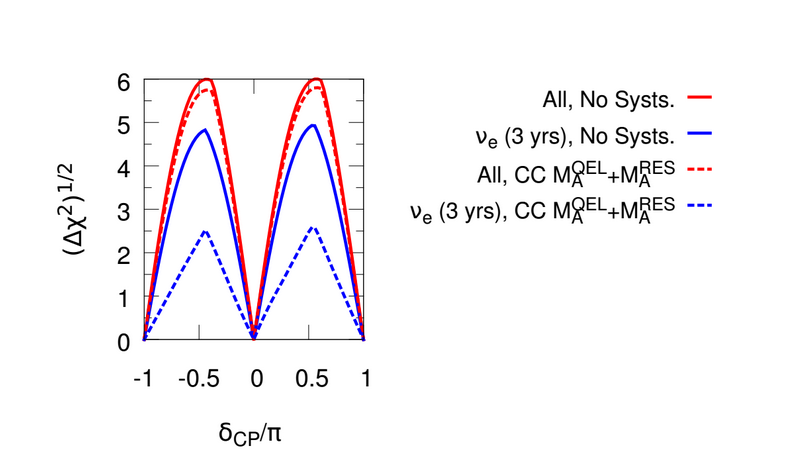
\includegraphics[width=0.8\linewidth]{figs/CPV_MARESQE.png}
% \caption{An example CP violation sensitivity calculated using inputs from the 
%   FastMC in a fit to all four ($\nu_e$, $\overline\nu_e$, $\nu_{\mu}$, 
%   $\overline\nu_{\mu}$) samples (red) and a fit to the $\nu_e$ appearance sample 
%   only (blue), for the case of no systematic uncertainty (solid) and the case in
%   which both $M_A^{QE,CC}$ and $M_A^{RES,CC}$ are allowed to vary with a
%   1$\sigma$ uncertainty of 20\% (dashed). This example was taken from an earlier
%   DUNE study, so the absolute sensitivity can not be compared with the DUNE 
%   sensitivities presented in this document.}
% \label{fig:MAresqesyst}
% \end{figure}

Uncertainty from nuclear interactions, in which particles exiting the primary
interaction vertex interact with the nuclear medium prior to depositing energy
in the detector, and detector effects, such as resolutions and energy scale
uncertainty, are somewhat more difficult to address with early simulation efforts.
However, in analogy to the treatment of cross-section uncertainty described above,
the effect of varying nuclear interaction parameters within their GENIE
uncertainties and comparisons of GENIE predictions to those of other
event generators are in progress.
Efforts to improve modeling of nuclear interactions and to develop 
reconstruction and analysis tools for a full Monte Carlo simulation are also underway. 
At the same time,
a number of test-beam and prototype experiments, including the DUNE 35-t prototype,
LARIAT, CAPTAIN, and the CERN neutrino platform experiments, are being designed and built to reduce these
uncertainties with experimental data.
